%& -shell-escape -enable-write18 
\documentclass[uplatex,dvipdfmx]{jsarticle}
\usepackage[utf8]{inputenc}

\usepackage[dvipdfmx]{graphicx}
\usepackage[dvipdfmx]{color}
\usepackage[driver=dvipdfm,hmargin=19.05truemm,vmargin=25.40truemm]{geometry}
\usepackage{colortbl}
\usepackage{tcolorbox}
\usepackage{varwidth}
\usepackage{xcolor}
\PassOptionsToPackage{dvipsnames}{xcolor}

\usepackage{amsmath,amsfonts,amssymb,amsthm}
\usepackage{bm}
\usepackage[italicdiff]{physics}
\usepackage{mathtools}
\mathtoolsset{showonlyrefs=true}
\usepackage[unicode, dvipdfmx]{hyperref}
\usepackage{pxjahyper}
\hypersetup{
setpagesize=false,
    bookmarksnumbered=true,
    bookmarksopen=true,
    colorlinks=true,
    linkcolor=cyan,
    citecolor=red,
}
\usepackage{mathrsfs}
\usepackage{bussproofs}
\usepackage{enumerate}
\usepackage{pxrubrica}
\usepackage{tipa}
\usepackage{ascmac}
\usepackage{caption}
\usepackage[subrefformat=parens]{subcaption}
\usepackage{listings,jvlisting}
\usepackage{tikz}
\usetikzlibrary{math,patterns,intersections,calc,arrows,graphs}
\usepackage{float}
\usepackage{xparse}
\usepackage{url}
\usepackage{fancyhdr}
\usepackage{multicol}
\usepackage{siunitx}
\usepackage{hhline}
\usepackage{bxbase}
\usepackage[mark=***]{sectionbreak}
\usepackage[geometry]{ifsym}
\usepackage[prefernoncjk]{pxcjkcat}
\usepackage[LGR,T2A,T3,T1]{fontenc}
\usepackage[greek,latin,english,russian,japanese]{pxbabel}

\allowdisplaybreaks


\theoremstyle{definition}
\newtheorem{theorem}{Thm}
\newtheorem{corollary}{Col}
\newtheorem{lemma}{Lem}
\newtheorem{definition}{Def}
\newtheorem{proposition}{Prop}

\tcbuselibrary{most}

\renewcommand{\labelitemi}{$\circ$}
\renewcommand{\labelitemii}{$\triangleright$}

\ProvideDocumentCommand\floor{m}{\lfloor {#1} \rfloor}
\ProvideDocumentCommand{\where}{}{\mathrel{}\middle|\mathrel{}}
\ProvideDocumentCommand{\when}{m}{\quad({#1})}
\ProvideDocumentCommand{\adjoint}{}{\mathbf{\ast}}
\ProvideDocumentCommand{\conjugation}{}{\mathbf{\ast}}
\NewDocumentCommand{\Jacobi}{m m}{\frac{\partial ({#1})}{\partial ({#2})}}
\NewDocumentCommand{\JacobiPolar}{O{x,y}}{\frac{\partial ({#1})}{\partial (r,\theta)}}
\DeclareMathOperator{\Ker}{Ker}
\DeclareMathOperator{\Img}{Im}
\DeclareMathOperator{\res}{Res}
\DeclareMathOperator{\Dom}{Dom}
\DeclareMathOperator{\Ran}{Ran}

\DeclareMathOperator{\exd}{d}

\DeclareFontShape{JY2}{mc}{m}{it}{<->ssub*mc/m/n}{}
\DeclareFontShape{JY2}{mc}{m}{sl}{<->ssub*mc/m/n}{}
\DeclareFontShape{JY2}{mc}{m}{sc}{<->ssub*mc/m/n}{}
\DeclareFontShape{JY2}{gt}{m}{it}{<->ssub*gt/m/n}{}
\DeclareFontShape{JY2}{gt}{m}{sl}{<->ssub*gt/m/n}{}
\DeclareFontShape{JY2}{mc}{b}{it}{<->ssub*mc/bx/it}{}
\DeclareFontShape{JY2}{mc}{bx}{it}{<->ssub*gt/m/n}{}
\DeclareFontShape{JY2}{mc}{bx}{sl}{<->ssub*gt/m/n}{}
\DeclareFontShape{JT2}{mc}{m}{it}{<->ssub*mc/m/n}{}
\DeclareFontShape{JT2}{mc}{m}{sl}{<->ssub*mc/m/n}{}
\DeclareFontShape{JT2}{mc}{m}{sc}{<->ssub*mc/m/n}{}
\DeclareFontShape{JT2}{gt}{m}{it}{<->ssub*gt/m/n}{}
\DeclareFontShape{JT2}{gt}{m}{sl}{<->ssub*gt/m/n}{}
\DeclareFontShape{JT2}{mc}{b}{it}{<->ssub*gt/b/n}{}
\DeclareFontShape{JT2}{mc}{bx}{it}{<->ssub*gt/m/n}{}
\DeclareFontShape{JT2}{mc}{bx}{sl}{<->ssub*gt/m/n}{}

\DeclareFontShape{J30}{mc}{b}{it}{<->ssub*mc/bx/it}{}
\DeclareFontShape{J30}{mc}{b}{n}{<->ssub*mc/bx/n}{}
\DeclareFontShape{J20}{mc}{b}{it}{<->ssub*mc/bx/it}{}
\DeclareFontShape{J20}{mc}{b}{n}{<->ssub*mc/bx/n}{}
\ProvideDocumentCommand{\titleof}{m}{

\title{ここに講義タイトルを入力 \\ {#1}レポート課題}
\author{ここに名前を入力}
\date{}
}
\titleof{11/02}

\begin{document}
    
\maketitle

\begin{enumerate}[(1)]
    \item 
    \begin{enumerate}[(i)]
        \item \ 
        \begin{itemize}
            \item $\displaystyle \int_1^\infty \frac{1}{x(\log x)^2}\dd{x}$は発散する.\\
            $a>1$として,
            \begin{gather}
                \lim_{s\to 1+0}\int_s^a \frac{1}{x(\log x)^2}\dd{x}, \lim_{t\to \infty}\int_a^t \frac{1}{x(\log x)^2}\dd{x}
            \end{gather}
            の収束発散を調べる.
            \begin{equation}
                \lim_{s\to 1+0}\int_s^a \frac{1}{x(\log x)^2}\dd{x}=\lim_{s\to 1+0}\eval[-\frac{1}{\log x}|_s^a = \infty
            \end{equation}
            は発散するので,$\displaystyle \int_1^\infty \frac{1}{x(\log x)^2}\dd{x}$は発散する.
            \item $\displaystyle \int_1^\infty \frac{\log x}{x^2}\dd{x}$は収束する.
            \begin{align}
                \int_1^\infty \frac{\log x}{x^2}\dd{x}
                &=\lim_{s\to\infty}\int_1^s\frac{\log x}{x^2}\dd{x}\\
                &=\lim_{s\to\infty}\qty{\eval[-\frac{1}{x}\log x|_{1}^{s}-\int_1^s-\frac{1}{x^2}\dd{x}}\\
                &=\lim_{s\to\infty}\qty{\eval[-\frac{\log x+1}{x}|_{1}^{s}}\\
                &=1
            \end{align}
            \item $\displaystyle \int_0^1 \frac{\log x}{x^2}\dd{x}$は発散する.
            \begin{align}
                \lim_{s\to +0}\int_s^1\frac{\log x}{x^2}\dd{x}
                &=\lim_{s\to +0}\eval[-\frac{\log x+1}{x}|_s^1\\
                &=-\infty\\
            \end{align}
            は発散する.
            \item $\displaystyle \int_0^{\frac{\pi}{2}} \frac{1}{\cos x}\dd{x}$は発散する.
            \begin{align}
                \int_0^{\frac{\pi}{2}} \frac{1}{\cos x}\dd{x}
                &=\lim_{t\to \frac{\pi}{2}-0}\int_0^{t} \frac{1}{\cos x}\dd{x}\\
                &=\frac{1}{2} \lim_{t\to \frac{\pi}{2}-0}\int_0^{t} (\cos x) \qty(\frac{1}{1-\sin x}+\frac{1}{1+\sin x}) \dd{x}\\
                &=\frac{1}{2} \lim_{t\to \frac{\pi}{2}-0} \eval[-\log\abs{1-\sin x}+\log\abs{1+\sin x}|_0^{t} \\
                &=\frac{1}{2} \lim_{s\to +0} \qty{-\log s+\log 2} = \infty
            \end{align}
            は発散する.
        \end{itemize}
        \item \
        \begin{itemize}
            \item $\displaystyle \sum_{n=2}^\infty \frac{1}{n(\log n)^2}$は収束する.\\
            $\dfrac{1}{x(\log x)^2}$は$x>1$で単調減少だから,$m>2$に対して
            \begin{align}
                \sum_{n=2}^m \frac{1}{n(\log n)^2} &<\frac{1}{2(\log 2)^2}+\int_2^m \frac{1}{x(\log x)^2}\\
                &\to \frac{1}{2(\log 2)^2} + \frac{1}{\log 2}\quad (m\to \infty)
            \end{align}
            \item $\displaystyle \sum_{n=2}^\infty \frac{\log n}{n^2}$は収束する.\\
            $\dfrac{\log x}{x^2}$は$x>\sqrt{e}$で単調減少だから,$m>2$に対して
            \begin{align}
                \sum_{n=2}^\infty \frac{\log n}{n^2}
                &< \frac{\log 2}{2^2}+\int_2^m \frac{\log x}{x^2}\dd{x}\\
                &\to \frac{1}{4}\log 2+\frac{\log 2 + 1}{2} \\
                &= \frac{3}{4}\log 2+\frac{1}{2} \\
            \end{align}
        \end{itemize}
    \end{enumerate}
    \item $n=3$である.
    \begin{align}
        \sum_{n=0}^3 I_n
        &=\int_0^\infty \frac{\displaystyle \sum_{n=0}^3 x^n}{(x^2+x+1)(x^3+x^2+x+1)}\dd{x}\\
        &=\int_0^\infty \frac{1}{x^2+x+1}\dd{x}\\
        &=\frac{2}{\sqrt{3}} \lim_{u\to\infty} \eval[\mathrm{Arctan}{\frac{2x+1}{\sqrt{3}}}|_0^\infty\\
        &=\frac{2}{\sqrt{3}} \qty(\frac{\pi }{2}-\frac{\pi}{6}) \\
        &=\frac{2\pi}{3\sqrt{3}}
    \end{align}
    である.
    \item 
    \begin{enumerate}[(i)]
        \item 
        \begin{proposition}
            そのような$\qty{a_n}$を与える関数として,
            \begin{equation}
                f(x)=
                \begin{dcases}
                    k-k^4\abs{x-k}&(\abs{x-k}\le \dfrac{1}{k^3}) \qq{($k = 1,2,\dots$)} \\
                    0&\qq{(otherwise)}
                \end{dcases}
            \end{equation}
            がある.
        \end{proposition}
        \begin{proof}
            $f(x)$が条件を満たすことの証明.\\
            ある$k$に対し,$\abs{x-k}=\dfrac{1}{k^3}$となるとき,
            \begin{align}
                f(x)
                &=k-k^4\cdot\frac{1}{k^3}\\
                &=k-k\\
                &=0
            \end{align}
            であるから,$f(x)$はこの点で連続である.\\
            それ以外の区間では$f(x)$は直線または折れ線なので,連続である.\\
            以上から条件(a)は満たされた.
            \begin{align}
                \int_0^\infty f(x)\dd{x}
                &=\sum_{n=2}^\infty \frac{1}{2}\cdot\frac{2}{n^3}\cdot n\\
                &=\sum_{n=2}^\infty \frac{1}{n^2}\\
                &=\frac{\pi^2}{6}-1
            \end{align}
            から条件(b)は満たされた.
        \end{proof}
        また,$\qty{a_n}_{n=0}^\infty=n$とすると,$\displaystyle\lim_{n\to\infty}a_n=\infty$であって
        \begin{align}
            \lim_{n\to\infty}f(a_n)
            &=\lim_{n\to\infty}{ n-n^4\cdot 0}\\
            &=\lim_{n\to\infty} n\\
            &=\infty
        \end{align}
        である.
        グラフは次のようになる.
        \begin{figure}[H]
            \centering
            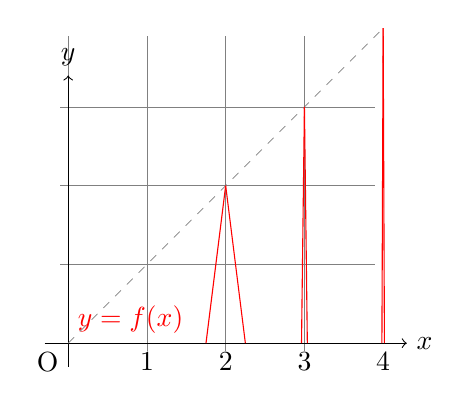
\begin{tikzpicture}[domain=0:4]

                \draw[very thin,color=gray] (-0.1,-0.1) grid (3.9,3.9);
                \draw[->] (-0.3,0) -- (4.3,0) node[right] {$x$};
                \draw[->] (0,-0.3) -- (0,3.4) node[above] {$y$};
                
                \draw (0,0) node[below left] {$\mathrm{O}$};
                \draw (1,0) node[below] {$1$};
                \draw (2,0) node[below] {$2$};
                \draw (3,0) node[below] {$3$};
                \draw (4,0) node[below] {$4$};

                \draw[domain=0:1.75,color=red] plot[id=0] function{0} ;
                \draw[domain=2.25:2.963,color=red] plot[id=0] function{0} ;
                \draw[domain=3.037:3.984,color=red] plot[id=0] function{0} ;
                \draw[domain=4.016:4.4,color=red] plot[id=0] function{0} node[above right] {$y=f(x)$};

                \draw[dashed,very thin,color=gray] (0,0) -- (4,4);

                \draw[color=red] (1.75,0) -- (2,2);
                \draw[color=red] (2.25,0) -- (2,2);

                \draw[color=red] (2.963,0) -- (3,3);
                \draw[color=red] (3.037,0) -- (3,3);

                \draw[color=red] (3.984,0) -- (4,4);
                \draw[color=red] (4.016,0) -- (4,4);
            \end{tikzpicture}
        \end{figure}
        \item {\color{blue} 証明を思いつきませんでした.対偶を考えれば示せそうだと思います.$f(b_n)$が0以外の値に収束するならば矛盾することは示せたので書きます.}\\
        $\displaystyle\lim_{x\to \infty}f(x)=\beta\quad(\beta>0)$であるとする.このとき,ある$\delta$が存在して
        \begin{equation}
            x>\delta\to \abs{f(x)-\beta}<\frac{\beta}{2}
        \end{equation}
        が成り立つ.$x>\delta$のとき,
        \begin{align}
            \abs{f(x)-\beta}&<\frac{\beta}{2}\\
            \therefore f(x)>\frac{\beta}{2}
        \end{align}
        となるから,関数
        \begin{equation}
            g(x)=
            \begin{dcases}
                \dfrac{\beta}{2}&(x>\delta)\\
                0&\qq{(otherwise)}
            \end{dcases}
        \end{equation}
        はつねに
        \begin{equation}
            f(x)>g(x)
        \end{equation}
        を満たしており,
        \begin{align}
            \int_0^\infty g(x)\dd{x}
            &=\lim_{u\to\infty}(u-\delta)\cdot\frac{\beta}{2}\\
            &=\infty
        \end{align}
        であるから
        \begin{equation}
            \int_0^\infty f(x)\dd{x}=\infty
        \end{equation}
        より矛盾.
    \end{enumerate}
\end{enumerate}

\end{document}